\section{Implementierung}
\label{sec:implementierung}

In diesem Abschnitt wird die Implementierung des in Abschnitt \ref{sec:konzept} vorgestellten Konzepts besprochen. Dazu werden als erstes die Voraussetzungen für das Ausführen der Anwendung und die Einrichtung der Server beschrieben (siehe Abschnitt \ref{sec:voraussetzungen}). Anschließend wird das Entwickelte Skript vorgestellt (siehe Abschnitt \ref{sec:setupskript}) und die dazu gehörige Konfigurations-Datei erläutert (siehe Abschnitt \ref{sec:konfigurationsdatei}). Zum Abschluss wird der Ablauf des Skripts erläutert (siehe Abschnitt \ref{sec:ablauf}).

\subsection{Voraussetzungen}
\label{sec:voraussetzungen}

Wie bereits teilweise in Abschnitt \ref{sec:grundlagen} beschrieben, benötigt man auf einem Webserver, der eine Wikipedia-Instanz bereitstellen soll, folgende Software:
\begin{itemize}
\item Webserver (empfohlen Apache httpd\footnote{\url{http://httpd.apache.org/}})
\item PHP (empfohlen $\geq$ 5.0)
\item MySQL (empfohlen $\geq$ 4.0)
\item ImageMagick (empfohlen zur Generierung von Thumbnails)
\end{itemize}

Außerdem wird auf dem Rechner, auf dem das Setup-Skript ausgeführt wird, mindestens Python 2.6 benötigt und gegebenenfalls \texttt{gnuplot}. Zudem muss ein Mediawiki\footnote{\url{http://www.mediawiki.org/}} installiert und der Wikipedia Dump in die Datenbank eingespielt sein. Auf den Servern, auf denen die Wikipedia Umgebung installiert werden soll, wird mindestens Python 2.4 benötigt.

In diesem konkreten Fall wurde die Mediawiki Version 1.16.5 genutzt und der Dump der Wikipedia Artikel zuerst mit dem Programm \texttt{xml2sql}\footnote{\url{http://meta.wikimedia.org/wiki/Xml2sql/}} in SQL transformiert und dann mit dem Programm \texttt{mysqlimport} in die Datenbank importiert. Dieses Verfahren wird offiziell nicht empfohlen, aber es stellte sich als schneller und sicherer heraus als die Nutzung des PHP Skripts vom Mediawiki.

Anschließend sollte die Datenbank in diesem Zustand gesichert werden, da dieser Stand der Datenbank wieder benötigt wird, falls ein anderer Abschnitt des Traces vorbereitet werden soll. Dazu sollte das MySQL Verzeichnis (z.B. \texttt{/var/lib/mysql/}) per \texttt{tar} gepackt werden und gegebenenfalls noch komprimiert werden per \texttt{gzip} oder \texttt{bzip2}. Dieses Archiv wird später bei der Konfiguration des Setup-Skripts benötigt.

Nach der Installation vom Mediawiki (der Ordner des Mediawiki sollte \glqq{}w/\grqq{} genannt werden) muss die Datei \texttt{LocalSettings.php} noch angepasst werden. Dazu sollten folgende Zeilen ergänzt werden:
\begin{verbatim}
$wgArticlePath      = '/wiki/$1';
$wgScriptPath       = "/w";

$wgMaxShellMemory   = "unlimited";
$wgMaxShellFileSize = "unlimited";

require_once( "$IP/extensions/Cite/Cite.php" );
require_once( "$IP/extensions/ImageMap/ImageMap.php" );
require_once( "$IP/extensions/OggHandler/OggHandler.php" );
require_once( "$IP/extensions/ParserFunctions/ParserFunctions.php" );
\end{verbatim}
Die angegeben Extensions müssen dann noch heruntergeladen werden und in dem \texttt{extensions} Ordner hinterlegt werden. Dies ist z.B. über das SVN-Repository\footnote{\url{http://svn.wikimedia.org/svnroot/mediawiki/tags/REL1_16_5/extensions/}} des Mediwiki möglich. Damit der Apache httpd Server mit den verschieden URL-Formen der Wikipedia zurecht kommt, sollte noch folgende Eintrag in der httpd-Konfigurationsdatei (welche z.B. unter  \texttt{/etc/httpd/conf/httpd.conf} zu finden ist) ergänzt werden (wobei der Pfad zur \texttt{index.php} anzupassen ist):
\begin{verbatim}
Alias /wiki "/var/www/html/w/index.php"
\end{verbatim}
Es gibt noch weitere Möglichkeiten die Unterstützung der Short-URLs von Wikipedia zu erreichen, diese sind in dem Mediawiki Wiki\footnote{\url{http://www.mediawiki.org/wiki/Manual:Short_URL}} nachzulesen.

Bei der Verwendung von RedHat basierten Systemen (wie z.B. CentOS) ist zu beachten, dass in dem Paket \texttt{gnome-vfs2} bis zur Version 2.16.2-8.el5 ein Bug\footnote{\url{http://rhn.redhat.com/errata/RHBA-2011-0441.html}} die korrekte Ausführung von ImageMagick verhindert. Dadurch konnten keine Thumbnails für SVG Dateien erstellt werden. Daher ist es empfehlenswerte mindestens die genannte Version des Pakets zu installieren.

\subsection{Setup-Skript}
\label{sec:setupskript}

Die entwickelte Anwendung ist ein Python 2.6 Skript \texttt{setup\_env.py} und nutzt das ebenfalls selbst entwickelte Modul \texttt{ppr}. Der Sourcecode liegt der Ausarbeitung bei oder kann aus einem GIT-Repository\footnote{\url{https://github.com/menski/ppr-s11}} heruntergeladen werden.

In Abbildung \ref{fig:classes} wird das Klassendiagramm des \texttt{ppr} Moduls gezeigt. Die Basisklasse \texttt{Process} erbt von der Klasse \texttt{multiprocessing.Process}. Daran ist zu erkennen das fast jede Klasse ebenfalls ein eigener Prozess ist. Somit können verschieden Aufgaben in dem Skript parallel durchgeführt werden. Die Kommunikation zwischen den Prozessen wird über sogenannte \texttt{Pipes} realisiert, wodurch Daten nicht lange im Speicher gehalten werden müssen.

\begin{figure}
  \centering
  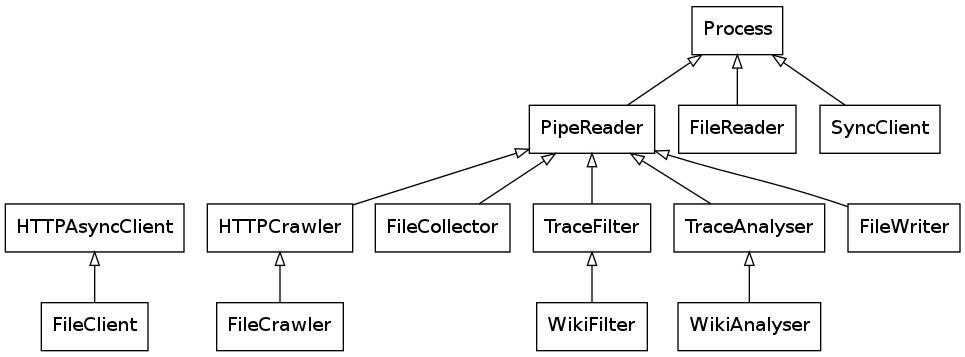
\includegraphics[width=\textwidth]{images/classes.png}
  \caption{Klassendiagramm des \texttt{ppr}-Moduls}
  \label{fig:classes}
\end{figure}

\subsubsection{Klassen}
\label{sec:klassen}

\begin{description}
\item[Process:] Basisklasse, welche von \texttt{multiprocessing.Process} erbt und eine Logger bereitstellt.
\item[SyncClient:] Ist eine Klasse, die genutzt wird um eine Wikipedia Instanz auf einen anderen Rechner zu kopieren.
\item[FileReader:] Diese Klasse liest eine Datei ein und sendet den Inhalt zur Verarbeitung an eine Menge von \texttt{Pipes}. Dabei ist es möglich die Funktion zum Öffnen der Datei anzugeben, um z.B. komprimierte Dateien zu öffnen.
\item[PipeReader:] Eine Klasse, welche eine \texttt{Pipe} nach Außen anbietet, über die sie mit Daten versorgt werden kann.
\item[FileWriter:] Erbt von der Klasse \texttt{PipeReader} und speichert die übergeben Daten in einer Datei. Wiederum ist es möglich eine Funktion zum Öffnen der Datei anzugeben, um z.B. komprimierten Dateien zu schreiben.
\item[TraceAnalyser/WikiAnalyser:] Spezielle \texttt{PipeReader} zur Analyse von Traces und zum Erstellen von Statistiken und Grafiken.
\item[TraceFilter/WikiFilter:] Klassen zum Filtern von Traces, welche ebenfalls von \texttt{PipeReader} erben.
\item[HTTPAsyncClient/FileClient:] Klassen, welche das Python Modul \texttt{asynchat} nutzen um HTTP1.1 Requests zu versenden. Die Klasse \texttt{FileClient} kann außerdem den Response in einer Datei speichern.
\item[HTTPCrawler/FileCrawler:] Klassen, die unter Nutzung der \texttt{HTTPAsyncClient/FileClient} Klassen und dem Python Modul \texttt{asyncore}, asynchrone HTTP Request versenden.
\item[FileCollector:] Eine Unterklasse von \texttt{PipeReader}, welche überprüft ob eine Datei bereits im Dateisystem existiert und falls nicht diese mit Hilfe der \texttt{FileCrawler} Klasse versucht herunterzuladen.
\end{description}

\subsubsection{Konfigurations-Datei}
\label{sec:konfigurationsdatei}

Ein vollständige Konfigurations-Datei ist im Anhang \ref{sec:konfiguration} aufgeführt. In diesem Abschnitt sollen die einzelnen Bereiche der Konfigurations-Datei erläutert werden.

\paragraph{[general]}

In dem \texttt{general} Abschnitt können die einzelnen Schritte des Skritps aktiviert bzw. deaktiviert werden (siehe dazu Abschnitt \ref{sec:konzept}). Außerdem kann das Log-Level gewählt werden und festgelegt werden ob bei der Analyse eine Grafik für die Requests pro Sekunde erstellt werden soll (dazu ist \texttt{gnuplot} nötig).

\paragraph{[trace]}

Der folgende \texttt{trace} Abschnitt gibt den Pfad zur Trace-Datei an und ob sie mit \texttt{gzip} komprimiert ist.

\paragraph{[filter]}

Im \texttt{filter} Abschnitt wird das Zeitintervall definiert, nach dem der Trace gefiltert wird. Dabei wird das Format $a:b$ genutzt und auf die folgende Weise interpretiert: $a$ ist ein UNIX-Zeitstempel, wenn $a > b$ gilt wird $b$ als Anzahl von Sekunden interpretiert und auf $a$ addiert, sonst wird $b$ ebenfalls als UNIX-Zeitstempel interpretiert. Als nächstes wird eine Hostname bestimmt, der genutzt wird um einen modifizierten Trace zu erstellen, welcher später zum Wiedereinspielen genutzt werden kann. Um nach bestimmten URLs zu filtern kann ein regulärer Ausdruck angegeben werden. Abschließend kann bestimmt werden, ob die gefilterten Traces mit \texttt{gzip} komprimiert gespeichert werden.

\paragraph{[download]}

Der \texttt{download} Abschnitt definiert das Verhalten beim Herunterladen von Bilder. Dazu wird ein Pfad angegeben, an dem nach bereits heruntergeladen Bilder gesucht wird und ebenfalls die neue heruntergeladenen Bilder gespeichert werden. Weiterhin kann der Port angegeben werden, über den die Requests versendet werden, um neue Bilder herunterzuladen. Die \texttt{async} Option gibt die parallel aufgebauten, asynchronen Verbindungen an. Des weiteren, werden die Pfade zu der Mediawiki- und MySQL-Installation, sowie der Name des lokal laufenden MySQL-Services benötigt. Mit den Optionen \texttt{clean\_images} und \texttt{clean\_mysql} kann bestimmt werden ob die aktuell in der Mediawiki-Installation vorhanden Bilder anfangs gelöscht werden sollen, bzw. ob die Datenbank vor dem einlesen der Bilder gelöscht werden soll und durch eine \glqq{}saubere\grqq{} Datenbank ersetzt werden soll. Diese \glqq{}saubere\grqq{} Datenbank wird über die Option \texttt{mysql\_archive} bestimmt. Die nach dem erfolgreichen Einrichten gepackten Mediawiki- und MySQL-Archive werden an dem Pfad gespeichert, der mit der Option \texttt{output\_dir} bestimmt wird.

\paragraph{[install]}

Der \texttt{install} Abschnitt ist der letzte notwendige Abschnitt. Er besteht allein aus einem String, welcher die Server angibt auf denen die Wikipedia-Instanz installiert werden soll und die dafür zu verwendende Konfiguration. Dabei ist der String eine durch \glqq{}:\grqq{} getrennte Liste. Jedes Element besteht aus einem Konfigurations-Namen, welcher durch ein \glqq{}@\grqq{} von einer einer Liste (getrennt durch Kommata) von IP-Adressen oder Hostname getrennt ist. Für jeden angegebenen Konfigurations-Namen muss wiederum ein Abschnitt in der Konfigurations-Datei angelegt werden. Diese Abschnitte bestehen dann aus dem Usernamen auf dem Server, dem Verzeichnis in, das die zu übertragenden Daten kopiert werden, dem Verzeichnis in dem das Mediawiki bzw. die MySQL-Datenbank installiert werden soll und dem Namen des MySQL-Service auf dem Server.

\subsubsection{Ablauf}
\label{sec:ablauf}
In diesem Abschnitt soll der Ablauf des Skripts dargestellt werden und beschrieben werden, welche Dateien erstellt werden.

\begin{enumerate}
\item Die Konfigurations-Datei wird eingelesen und auf Korrektheit geprüft.
\item Sofern der Analyse-Schritt oder Filter-Schritt aktiviert wurde, wird ein \texttt{FileReader} für das Tracefile erzeugt. Ist eine Analyse gefordert wird ein \texttt{WikiAnalyser} erzeugt bzw. ist die Filterung gefordert ein \texttt{WikiFilter}. Der \texttt{FileReader} sendet nun die gelesen Daten an die erzeugten Instanzen. Wurde eine \texttt{WikiAnalyser} erzeugt, erstellt dieser für eine Trace-Datei \texttt{trace.gz}, die folgenden Dateien:
  \begin{itemize}
  \item \texttt{trace.gz.stats} (Statistiken zum Trace)
  \item \texttt{trace.image.gz} (Alle Requests, die ein Bild anfordern)
  \item \texttt{trace.thumb.gz} (Alle Requests, die ein Thumbnail anfordern)
  \item \texttt{trace.page.gz} (Alle restlichen Requests)
  \item \texttt{trace.gz.eps} und \texttt{trace.gz.log} (falls die \texttt{plot} Option aktiviert wurde; Requests pro Sekunde Graph und gnuplot Ausgabe)
  \end{itemize}
Eine \texttt{WikiFilter} Instanz erzeugt die Dateien \texttt{trace.timestampA-timestampB.gz} (gefilterter Trace) sowie \texttt{trace.timestampA-timestampB.rewrite.gz} (Trace zum Wiedereinspielen). Außerdem erzeugt sie eine \texttt{WikiAnalyser} Instanz, womit ebenfalls für den gefilterten Trace, die oben beschrieben Datei erzeugt werden.
\item Im nächsten Schritt wird, sofern gewünscht, zuerst das Bilder-Verzeichnis von der Mediawiki-Installation geleert. Dann wird jeweils ein \texttt{FileReader} und ein \texttt{File\-Collector} für die benötigten Bilder bzw. Thumbnails erzeugt. Nachdem der Download abgeschlossen ist wird die Mediawiki-Installation gepackt und parallel die Bilder in die MySQL-Datenbank eingelesen und die MySQL-Datenbank ebenfalls gepackt.
\item Im letzten Schritt wird nun für jeden Server auf dem die Wikipedia-Instanz eingespielt werden soll, ein \texttt{SyncClient} erzeugt, der die gepackte MediaWiki-Installation, die gepackte MySQL-Datenbank und die Datei \texttt{ppr/server.py}, mittels \texttt{scp}, auf den entsprechenden Server kopiert. Und anschließend die kopierte Datei \texttt{server.py} mit entsprechenden Parametern über \texttt{ssh} aufruft. Das \texttt{server.py} Skript, welches wie bereits erwähnt Python 2.4 benötigt, entpackt die kopierten Archive auf dem Server und richtet die Umgebung ein. Anschließend ist auf dem Server die gewünschte Wikipedia-Instanz eingerichtet.
\end{enumerate}

\section{Beispiel: Trace-Analyse und -Filterung}
\label{sec:beispiel}

Die Trace-Analyse und -Filterung soll in diesem Kapitel anhand eines Beispiel Traces gezeigt werden. Dazu wurde die Trace-Datei \texttt{wiki.1194899823.gz}\footnote{\url{http://www.wikibench.eu/wiki/2007-11/wiki.1194899823.gz}} gewählt. Die Analyse dieses Traces ergibt die in Tabelle \ref{tab:trace-full} dargestellten Werte und der Verlauf der Requests pro Sekunde wird in Abbildung \ref{fig:trace-full} gezeigten. Filtert man diesen Trace nun für das Intervall 1194892290-1194894090 und nach den englischen Artikeln, erhält meinen einen Trace der durch die Tabelle \ref{tab:trace-filtered} und die Abbildung \ref{fig:trace-filtered} beschrieben wird. Es ist zu erkennen das der größte Teil der Requests Medien-Dateien abruft, welche über den Host \texttt{upload.wikimedia.org} erreichbar sind. Bei dem Abruf von Wikipedia Artikeln dominiert klar die englische Wikipedia und die Requests, welche mit \glqq{}save\grqq{} gekennzeichnet sind, können vernachlässigt werden.

\begin{table}
  \centering
  \begin{tabular}{|rr|}\hline
    \textbf{General} & \\\hline
    tracefile: & wiki.1194899823.gz \\
    start time: & Mon, 12 Nov 2007 18:31:30 +0000 \\
    end time: & Mon, 12 Nov 2007 19:31:35 +0000 \\
    duration: & 3604.986 sec \\
    lines: & 17.518.902 \\
    requests: & 17.518.817 \\
    page requests: & 7969566 (45,5\%) \\
    media requests: & 9.549.251 (54,5\%) \\
    errors: & 85 \\
    save operations: & 3.309 (0,02\%)\\\hline\hline
    \textbf{Hosts} & \\\hline
    upload.wikimedia.org: & 9.549.251 (54,5\%) \\
    en.wikipedia.org:&  3.228.167 (18,4\%) \\
    meta.wikimedia.org: &  977.302 (5,6\%) \\
    de.wikipedia.org:  & 747.068 (4,2\%)\\\hline
  \end{tabular}
  \caption{Trace-Analyse der Datei \texttt{wiki.1194899823.gz}}
  \label{tab:trace-full}
\end{table}

\begin{figure}
  \centering
  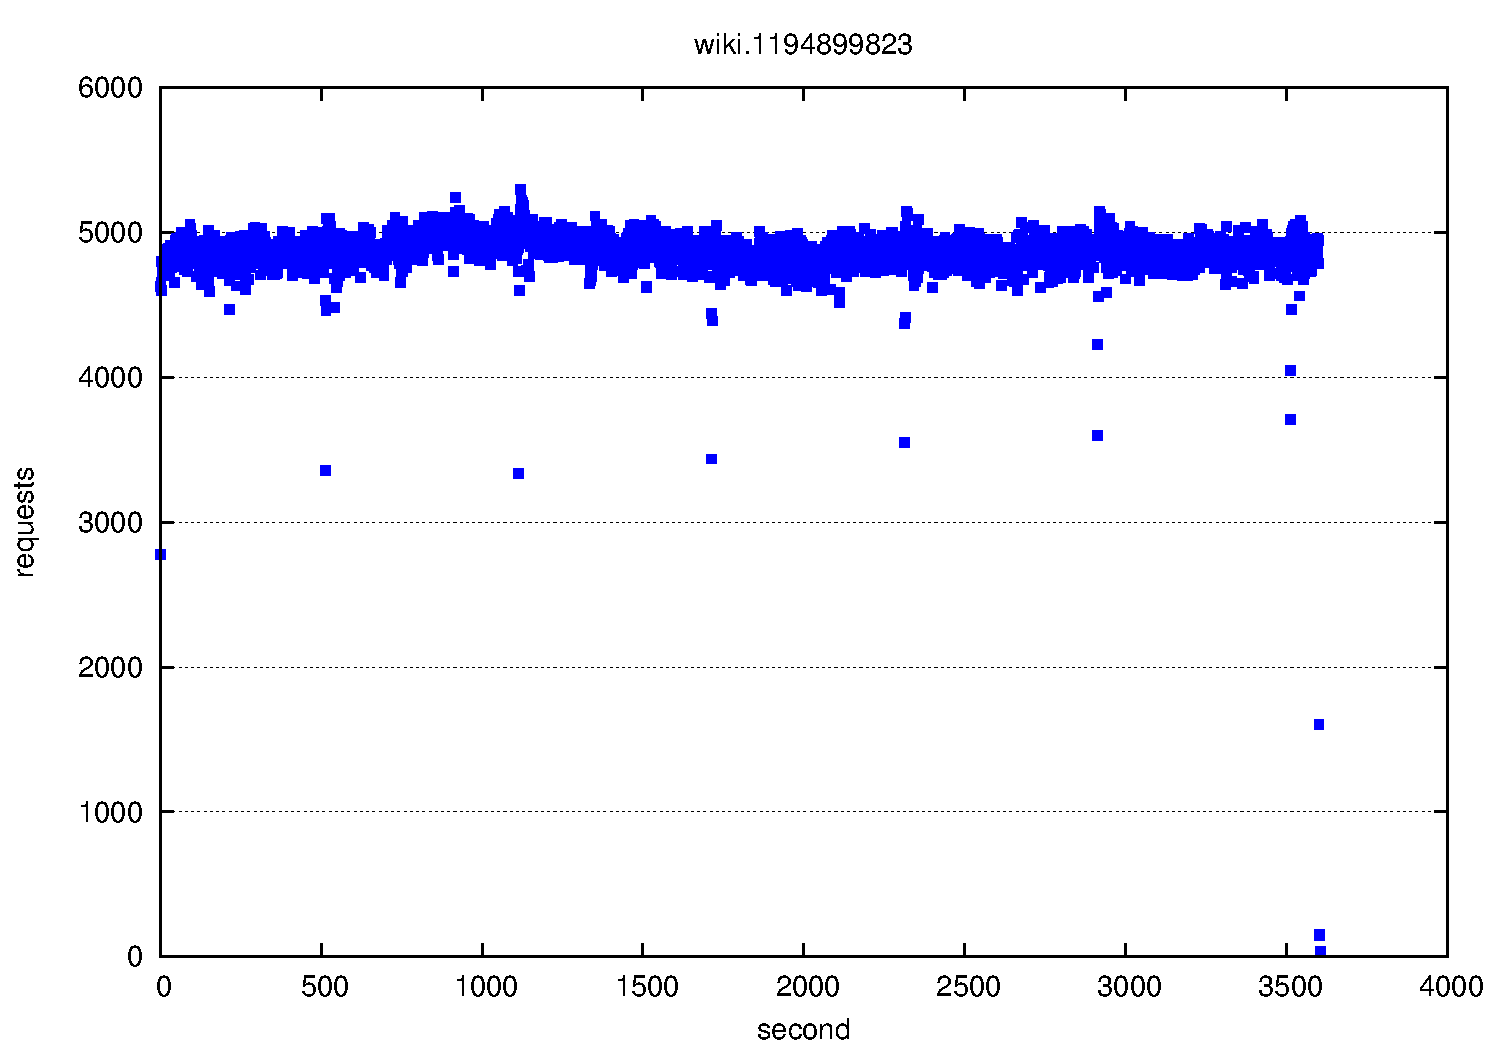
\includegraphics[width=\textwidth]{images/trace-full}
  \caption{Requests pro Sekunde der Datei \texttt{wiki.1194899823.gz}}
  \label{fig:trace-full}
\end{figure}

\begin{table}
  \centering
  \begin{tabular}{|rr|}\hline
    \textbf{General} & \\\hline
    tracefile: & wiki.1194899823.1194892290-1194894090.gz\\
    start time: & Mon, 12 Nov 2007 18:31:30 +0000\\
    end time: & Mon, 12 Nov 2007 19:01:30 +0000\\
    duration: & 1800.788 sec\\
    lines: & 4795845\\
    requests: & 4.795.845\\
    page requests: & 1.599.427 (33,3\%) \\
    media requests: & 3.196.418 (66,6\%) \\
    errors: & 0\\\hline\hline
    \textbf{Hosts} & \\\hline
    upload.wikimedia.org: & 3.196.418 (66,6\%) \\
    en.wikipedia.org: & 1.599.427 (33,3\%) \\\hline
  \end{tabular}
  \caption{Trace-Analyse der Datei \texttt{wiki.1194892290-1194894090.1194899823.gz}}
  \label{tab:trace-filtered}
\end{table}

\begin{figure}
  \centering
  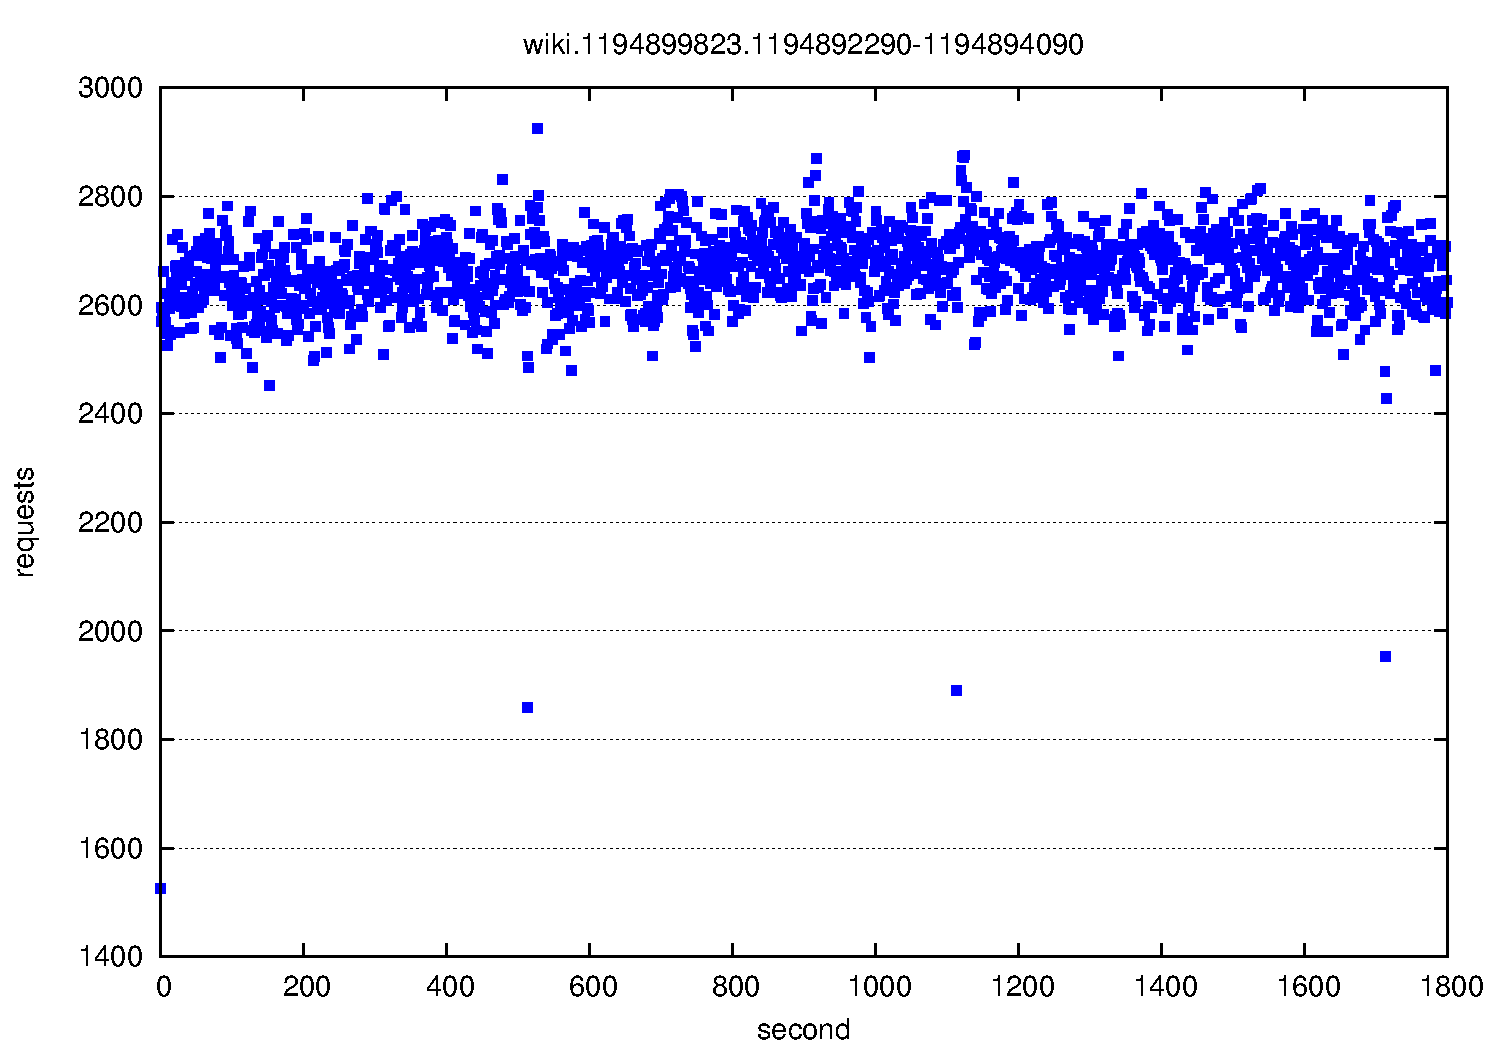
\includegraphics[width=\textwidth]{images/trace-filtered}
  \caption{Requests pro Sekunde der Datei \texttt{wiki.1194892290-1194894090.1194899823.gz}}
  \label{fig:trace-filtered}
\end{figure}

%%% Local Variables: 
%%% mode: latex
%%% TeX-master: "../master"
%%% End: 
